% MORPH — Retention (Gated Linear Attention) Memory
% The GLA branch and its TWO recurrence axes:
%   Axis 1 — over the SEQUENCE  (the SSM hidden state S_t, standard linear attention)
%   Axis 2 — over the LOOP      (S_T of iter i seeds iter i+1 — the cross-iteration carry)
% Relative vertical stacking (below=of) so panels resize without colliding.
% Compile: pdflatex morph_memory.tex

\documentclass[border=18pt]{standalone}
\usepackage[T1]{fontenc}
\usepackage{amsmath,amssymb}
\usepackage{tikz}
\usetikzlibrary{arrows.meta, positioning, calc, backgrounds, fit,
  decorations.pathreplacing}

% ── Colorblind-safe palette ─────────────────────────────────────
\definecolor{cbBlue}{HTML}{4477AA}
\definecolor{cbPurple}{HTML}{AA3377}
\definecolor{cbTeal}{HTML}{228833}
\definecolor{cbOrange}{HTML}{EE7733}
\definecolor{fBlue}{HTML}{DCEAF7}
\definecolor{fPurple}{HTML}{F0DCF0}
\definecolor{fTeal}{HTML}{D4EDDA}
\definecolor{fOrange}{HTML}{FDE8D0}
\definecolor{bdr}{HTML}{333333}
\definecolor{loopC}{HTML}{2255AA}

\tikzset{
  bigA/.style={-{Stealth[length=4mm,width=3mm]}, line width=2pt},
  A/.style={-{Stealth[length=2.8mm,width=2.2mm]}, thick},
  st/.style={draw=cbPurple, very thick, rounded corners=4pt, fill=fPurple,
    minimum width=1.7cm, minimum height=1.25cm, font=\normalsize\sffamily\bfseries,
    text=cbPurple!55!black, align=center},
  box/.style={draw=#1, thick, rounded corners=5pt, align=center,
    inner sep=7pt, font=\normalsize\sffamily},
  panel/.style={draw=#1, very thick, rounded corners=8pt,
    minimum width=15.6cm, anchor=north, inner sep=0pt},
  sub/.style={font=\footnotesize\sffamily},
  lbl/.style={font=\scriptsize\sffamily},
}

\begin{document}
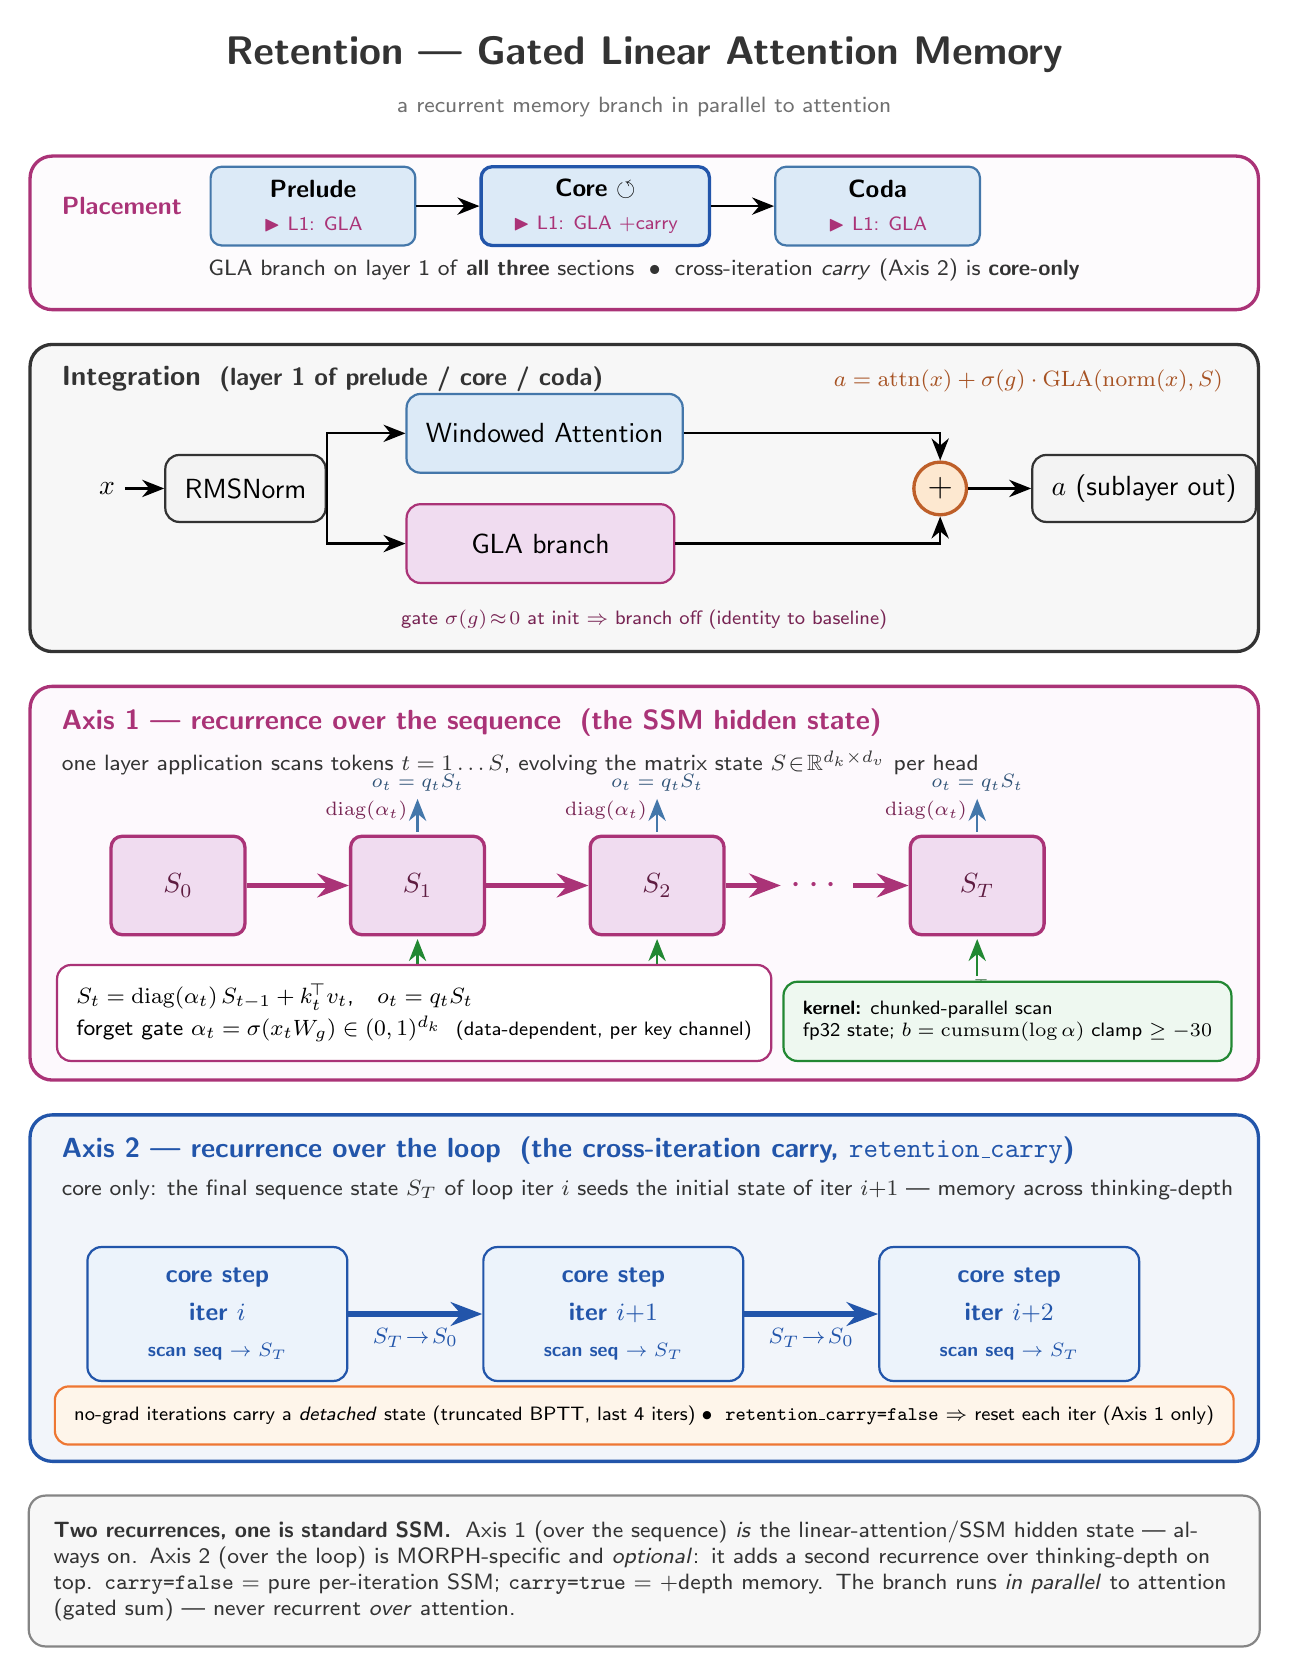
\begin{tikzpicture}[font=\sffamily, node distance=0.4cm]

% ── Title ───────────────────────────────────────────────────────
\node[font=\Large\sffamily\bfseries, text=bdr] (title) at (8.3,0)
  {Retention --- Gated Linear Attention Memory};
\node[sub, text=bdr!70, below=2pt of title] (subt)
  {a recurrent memory branch in parallel to attention};

% ════════════════════════════════════════════════════════════════
% PLACEMENT — the GLA branch lives in layer 1 of ALL THREE sections
% ════════════════════════════════════════════════════════════════
\node[panel=cbPurple, fill=fPurple, fill opacity=0.10,
      minimum height=1.95cm, below=0.35cm of subt] (place) {};
\node[font=\small\sffamily\bfseries, text=cbPurple, anchor=west]
  at ($(place.west)+(0.3,0.34)$) {Placement};
\node[draw=cbBlue, thick, rounded corners=4pt, fill=fBlue, minimum width=2.6cm,
      minimum height=1.0cm, font=\small\sffamily, align=center, anchor=west]
      (cpre) at ($(place.west)+(2.3,0.34)$)
      {\textbf{Prelude}\\[1pt]{\scriptsize \textcolor{cbPurple}{$\blacktriangleright$ L1: GLA}}};
\node[draw=loopC, very thick, rounded corners=4pt, fill=fBlue, minimum width=2.9cm,
      minimum height=1.0cm, font=\small\sffamily, align=center, right=0.8cm of cpre] (ccore)
      {\textbf{Core} $\circlearrowleft$\\[1pt]{\scriptsize \textcolor{cbPurple}{$\blacktriangleright$ L1: GLA $+$carry}}};
\node[draw=cbBlue, thick, rounded corners=4pt, fill=fBlue, minimum width=2.6cm,
      minimum height=1.0cm, font=\small\sffamily, align=center, right=0.8cm of ccore] (ccoda)
      {\textbf{Coda}\\[1pt]{\scriptsize \textcolor{cbPurple}{$\blacktriangleright$ L1: GLA}}};
\draw[A] (cpre) -- (ccore);
\draw[A] (ccore) -- (ccoda);
\node[sub, text=bdr, anchor=south] at ($(place.south)+(0,0.26)$)
  {GLA branch on layer 1 of \textbf{all three} sections \;$\bullet$\; cross-iteration \emph{carry} (Axis 2) is \textbf{core-only}};

% ════════════════════════════════════════════════════════════════
% INTEGRATION — parallel gated branch in the layer-1 block
% ════════════════════════════════════════════════════════════════
\node[panel=bdr, fill=bdr!4, minimum height=3.9cm, below=0.4cm of place] (intg) {};
\node[font=\normalsize\sffamily\bfseries, text=bdr, anchor=north west]
  at ($(intg.north west)+(0.3,-0.18)$)
  {Integration \;{\small (layer 1 of prelude / core / coda)}};
\node[sub, text=cbOrange!70!black, anchor=north east] at ($(intg.north east)+(-0.35,-0.22)$)
  {$a=\mathrm{attn}(x)+\sigma(g)\cdot\mathrm{GLA}(\mathrm{norm}(x),S)$};

\node[font=\normalsize\sffamily] at ($(intg.north west)+(1.0,-1.85)$) (xin) {$x$};
\node[box=bdr, fill=bdr!6, minimum height=0.85cm, right=0.5cm of xin] (rn) {RMSNorm};
\node[box=cbBlue, fill=fBlue, minimum height=1.0cm, minimum width=3.4cm,
      right=1.0cm of rn, yshift=0.7cm] (att) {Windowed Attention};
\node[box=cbPurple, fill=fPurple, minimum height=1.0cm, minimum width=3.4cm,
      right=1.0cm of rn, yshift=-0.7cm] (glab) {GLA branch};
\node[draw=cbOrange!80!black, very thick, circle, fill=fOrange, inner sep=2.5pt,
      right=2.9cm of att, yshift=-0.7cm, font=\large] (sum) {$+$};
\node[box=bdr, fill=bdr!6, minimum height=0.85cm, right=0.8cm of sum] (aout) {$a$ (sublayer out)};

\draw[A] (xin) -- (rn);
\draw[A] (rn.east) |- (att.west);
\draw[A] (rn.east) |- (glab.west);
\draw[A] (att.east) -| (sum);
\draw[A] (glab.east) -| (sum);
\draw[A] (sum) -- (aout);
\node[lbl, text=cbPurple!70!black, anchor=south] at ($(intg.south)+(0,0.18)$)
  {gate $\sigma(g)\!\approx\!0$ at init $\Rightarrow$ branch off (identity to baseline)};

% ════════════════════════════════════════════════════════════════
% AXIS 1 — recurrence over the SEQUENCE  (the SSM)
% ════════════════════════════════════════════════════════════════
\node[panel=cbPurple, fill=fPurple, fill opacity=0.16,
      minimum height=5.0cm, below=0.4cm of intg] (ax1) {};
\node[font=\normalsize\sffamily\bfseries, text=cbPurple, anchor=north west]
  at ($(ax1.north west)+(0.3,-0.18)$)
  {Axis 1 --- recurrence over the \emph{sequence}\; (the SSM hidden state)};
\node[sub, text=bdr, anchor=north west] at ($(ax1.north west)+(0.3,-0.72)$)
  {one layer application scans tokens $t=1\dots S$, evolving the matrix state
   $S\!\in\!\mathbb{R}^{d_k\times d_v}$ per head};

% state chain (relative to the panel)
\node[st] at ($(ax1.north west)+(1.9,-2.55)$) (S0) {$S_0$};
\node[st, right=1.3cm of S0] (S1) {$S_1$};
\node[st, right=1.3cm of S1] (S2) {$S_2$};
\node[font=\Large\sffamily\bfseries, text=cbPurple, right=0.7cm of S2] (dots) {$\cdots$};
\node[st, right=0.7cm of dots] (ST) {$S_T$};

\foreach \a/\b in {S0/S1, S1/S2, S2/dots, dots/ST}{
  \draw[bigA, cbPurple] (\a) -- (\b);}
\foreach \n in {S1,S2,ST}{
  \node[lbl, text=cbPurple!70!black] at ($(\n)+(-0.65,0.95)$) {$\mathrm{diag}(\alpha_t)$};
  \draw[A, cbTeal] ($(\n)+(0,-1.15)$) -- ($(\n)+(0,-0.68)$);
  \node[lbl, text=cbTeal!60!black] at ($(\n)+(0,-1.35)$) {$+\,k_t^{\!\top} v_t$};
  \draw[A, cbBlue] ($(\n)+(0,0.68)$) -- ($(\n)+(0,1.1)$);
  \node[lbl, text=cbBlue!70!black] at ($(\n)+(0,1.3)$) {$o_t=q_t S_t$};}

\node[box=cbPurple, fill=white, anchor=south west, font=\footnotesize\sffamily, align=left]
  at ($(ax1.south west)+(0.35,0.25)$) {%
  $S_t=\mathrm{diag}(\alpha_t)\,S_{t-1}+k_t^{\!\top} v_t$,\quad $o_t=q_t S_t$\\[2pt]
  forget gate $\alpha_t=\sigma(x_t W_g)\in(0,1)^{d_k}$ \;{\scriptsize (data-dependent, per key channel)}};
\node[box=cbTeal, fill=fTeal!40, anchor=south east, font=\scriptsize\sffamily, align=left]
  at ($(ax1.south east)+(-0.35,0.25)$) {%
  \textbf{kernel:} chunked-parallel scan\\
  fp32 state; $b=\mathrm{cumsum}(\log\alpha)$ clamp $\ge-30$};

% ════════════════════════════════════════════════════════════════
% AXIS 2 — recurrence over the LOOP  (the cross-iteration carry)
% ════════════════════════════════════════════════════════════════
\node[panel=loopC, fill=loopC!6,
      minimum height=4.4cm, below=0.4cm of ax1] (ax2) {};
\node[font=\normalsize\sffamily\bfseries, text=loopC, anchor=north west]
  at ($(ax2.north west)+(0.3,-0.18)$)
  {Axis 2 --- recurrence over the \emph{loop} \;(the cross-iteration carry, \texttt{retention\_carry})};
\node[sub, text=bdr, anchor=north west] at ($(ax2.north west)+(0.3,-0.72)$)
  {core only: the final sequence state $S_T$ of loop iter $i$ seeds the initial state of iter $i{+}1$
   --- memory across thinking-depth};

\node[draw=loopC, thick, rounded corners=5pt, fill=fBlue!55,
      minimum width=3.3cm, minimum height=1.7cm, font=\small\sffamily\bfseries,
      text=loopC, align=center] at ($(ax2.north west)+(2.4,-2.55)$) (it1)
      {core step\\[3pt]{\small iter $i$}\\[2pt]{\scriptsize scan seq $\to S_T$}};
\node[draw=loopC, thick, rounded corners=5pt, fill=fBlue!55,
      minimum width=3.3cm, minimum height=1.7cm, font=\small\sffamily\bfseries,
      text=loopC, align=center, right=1.7cm of it1] (it2)
      {core step\\[3pt]{\small iter $i{+}1$}\\[2pt]{\scriptsize scan seq $\to S_T$}};
\node[draw=loopC, thick, rounded corners=5pt, fill=fBlue!55,
      minimum width=3.3cm, minimum height=1.7cm, font=\small\sffamily\bfseries,
      text=loopC, align=center, right=1.7cm of it2] (it3)
      {core step\\[3pt]{\small iter $i{+}2$}\\[2pt]{\scriptsize scan seq $\to S_T$}};
\draw[bigA, loopC] (it1.east) -- (it2.west) node[midway, below=1pt, sub, text=loopC]{$S_T\!\to\!S_0$};
\draw[bigA, loopC] (it2.east) -- (it3.west) node[midway, below=1pt, sub, text=loopC]{$S_T\!\to\!S_0$};
\node[box=cbOrange, fill=fOrange!45, anchor=south, font=\scriptsize\sffamily, align=center,
      minimum width=8cm] at ($(ax2.south)+(0,0.22)$) {%
  no-grad iterations carry a \emph{detached} state (truncated BPTT, last 4 iters)\;$\bullet$\;
  \texttt{retention\_carry=false} $\Rightarrow$ reset each iter (Axis 1 only)};

% ════════════════════════════════════════════════════════════════
% FOOTER — the conceptual crux
% ════════════════════════════════════════════════════════════════
\node[draw=bdr!60, thick, rounded corners=6pt, fill=bdr!4, anchor=north,
      text width=15.0cm, inner sep=9pt, align=left, font=\footnotesize\sffamily, text=bdr,
      below=0.4cm of ax2] {%
  \textbf{Two recurrences, one is standard SSM.}\;
  Axis 1 (over the sequence) \emph{is} the linear-attention/SSM hidden state --- always on.
  Axis 2 (over the loop) is MORPH-specific and \emph{optional}: it adds a second recurrence over
  thinking-depth on top. \texttt{carry=false} $=$ pure per-iteration SSM; \texttt{carry=true} $=$ $+$depth memory.
  The branch runs \emph{in parallel} to attention (gated sum) --- never recurrent \emph{over} attention.};

\end{tikzpicture}
\end{document}
